\documentclass[11pt,letterpaper,twoside]{article}
\usepackage[tmargin=1in,bmargin=1in,lmargin=1in,rmargin=1in]{geometry}
\usepackage{../style/packages}
\usepackage{../style/commands}
\setbool{notesonly}{false}

% -------------------
% Content
% -------------------
\begin{document}

% Cover Photo
% !TEX root = ../main/aws_iwasawa.tex

\thispagestyle{empty}
\newgeometry{
	top=0cm, 
	bottom=0cm, 
	left=0cm, 
	right=0cm
}


\tikz[remember picture,overlay] \node[opacity=1,inner sep=0pt] at (current page.center){
\includegraphics[width=\paperwidth,height=\paperheight]{../cover/swc_poster.jpg}};

\phantom{x} % To image is placed.

% Reset Page Style
\newgeometry{
	top= 1in, 
	bottom= 1in, 
	left= 1in, 
	right= 1in
}
\newpage

% Cover
% !TEX root = ../main/aws_iwasawa.tex

\thispagestyle{empty}
\begin{flushright}
\begin{tabular}{ll}
\raisebox{-.5\height}{
\includegraphics[scale=0.055]{../cover/arizona_seal.png}} & {\color{ArzBlue} \Huge University of Arizona} 
\end{tabular}
\end{flushright}
\vspace{2in}

{%
\color{ArzRed} \Huge \noindent Arizona Winter School 2018 \par \Huge \noindent \color{ArzRed} Iwasawa Theory \par \color{ArzBlue}
\noindent \rule{0.70\textwidth}{0.05cm}
}

{\color{ArzBlue} \large \noindent Notes By: Caleb McWhorter }

\vfill
\begin{center} {\color{ArzBlue}\huge March 2018} \end{center}
\newpage

% TOC
\thispagestyle{blank}
\tableofcontents
\newpage

% -------------------
% Lectures
% -------------------

% Lecture Notes
\thispagestyle{empty}
\part{Talk Notes} 
    \newpage 
	\setcounter{page}{1}

% Greenberg
% !TEX root = ../../../main/aws_iwasawa.tex
\newpage
\section{Name: Lecture Title}
\subsection{Lecture 1}
\subsubsection{Lecture Name}

% Coates
% !TEX root = ../../../main/aws_iwasawa.tex
\newpage
\section{John Coates: Classical algebraic Iwasawa theory}
\subsection{Lecture 1}

$[F:\Q]<\infty$, $F_\infty/F$, $\Gamma=\gal(F_\infty/F)$

$\Gamma \xrightarrow{\sim} \Z_p$, $\Gamma_n \xrightarrow{\sim} p^n \Z_p$,

$F_\infty^{\Gamma_n}=F_n$, $\gal(F_n/F)=\Z/p^n\Z$

$F=F_0 \subset F_1 \subset \cdots \subset F_n \subset \cdots F_\infty= \cup F_n$

\underline{Facet 1}. $F_\infty/F$

Classical Iwasawa Theory: $p$-adic behavior of ideal class groups and units in $F_\infty/F$, and interpretation via global class field theory. 

$\zeta(s)= \prod_p (1-p^{-s})^{-1}$
\begin{enumerate}[(a)]
\item Complex zeros of $\zeta(s)$ $\leftrightarrow$ distribution of prime numbers.
\item $\zeta(1-n) \in \Q(n=2,4,6,\ldots)$
\end{enumerate}

Kummer $\leftrightarrow$ class number of $\Q(\mu_p)^+$

Leopoldt-Kubota: $p$-adic analogue of $\zeta(s)$.

Iwasawa: zeroes of $p$-adic analogue of $\zeta(s)$ $\leftrightarrow$ classical Iwasawa Theory of $\Q(\mu_p^{\infty})^+/\Q(\mu_p)^+$.
% !TEX root = ../../../main/aws_iwasawa.tex
\newpage
\section{Name: Lecture Title}
\subsection{Lecture 1}
\subsubsection{Lecture Name}
% !TEX root = ../../../main/aws_iwasawa.tex
\newpage
\section{Name: Lecture Title}
\subsection{Lecture 1}
\subsubsection{Lecture Name}
% !TEX root = ../../../main/aws_iwasawa.tex
\newpage
\section{Name: Lecture Title}
\subsection{Lecture 1}
\subsubsection{Lecture Name}

% Loeffler/Zerbes
% !TEX root = ../../../main/aws_iwasawa.tex
\newpage
\section{Name: Lecture Title}
\subsection{Lecture 1}
\subsubsection{Lecture Name}
% !TEX root = ../../../main/aws_iwasawa.tex
\newpage
\section{Name: Lecture Title}
\subsection{Lecture 1}
\subsubsection{Lecture Name}
% !TEX root = ../../../main/aws_iwasawa.tex
\newpage
\section{Name: Lecture Title}
\subsection{Lecture 1}
\subsubsection{Lecture Name}
% !TEX root = ../../../main/aws_iwasawa.tex
\newpage
\section{Name: Lecture Title}
\subsection{Lecture 1}
\subsubsection{Lecture Name}

% Sharifi
% !TEX root = ../../../main/aws_iwasawa.tex
\newpage
\section{Name: Lecture Title}
\subsection{Lecture 1}
\subsubsection{Lecture Name}
% !TEX root = ../../../main/aws_iwasawa.tex
\newpage
\section{Name: Lecture Title}
\subsection{Lecture 1}
\subsubsection{Lecture Name}
% !TEX root = ../../../main/aws_iwasawa.tex
\newpage
\section{Name: Lecture Title}
\subsection{Lecture 1}
\subsubsection{Lecture Name}
% !TEX root = ../../../main/aws_iwasawa.tex
\newpage
\section{Name: Lecture Title}
\subsection{Lecture 1}
\subsubsection{Lecture Name}

% Skinner
% !TEX root = ../../../main/aws_iwasawa.tex
\newpage
\section{Name: Lecture Title}
\subsection{Lecture 1}
\subsubsection{Lecture Name}
% !TEX root = ../../../main/aws_iwasawa.tex
\newpage
\section{Name: Lecture Title}
\subsection{Lecture 1}
\subsubsection{Lecture Name}
% !TEX root = ../../../main/aws_iwasawa.tex
\newpage
\section{Name: Lecture Title}
\subsection{Lecture 1}
\subsubsection{Lecture Name}
% !TEX root = ../../../main/aws_iwasawa.tex
\newpage
\section{Name: Lecture Title}
\subsection{Lecture 1}
\subsubsection{Lecture Name}
% !TEX root = ../../../main/aws_iwasawa.tex
\newpage
\section{Name: Lecture Title}
\subsection{Lecture 1}
\subsubsection{Lecture Name}


% -------------------
% Course/Project Outlines
% -------------------
\ifbool{notesonly}{}{%
\newpage
\thispagestyle{empty}
\part{Course/Project Outlines \& Lecture Notes}
\newpage

%\setcounter{section}{1}

% Coates
\phantomsection
\addtocounter{section}{1}
\addcontentsline{toc}{section}{\protect\numberline{\thesection} John Coates: Classical algebraic Iwasawa Theory}
\phantomsection
\setcounter{subsection}{1}
\addcontentsline{toc}{subsection}{\protect\numberline{\thesubsection} Course \& Project Outline}
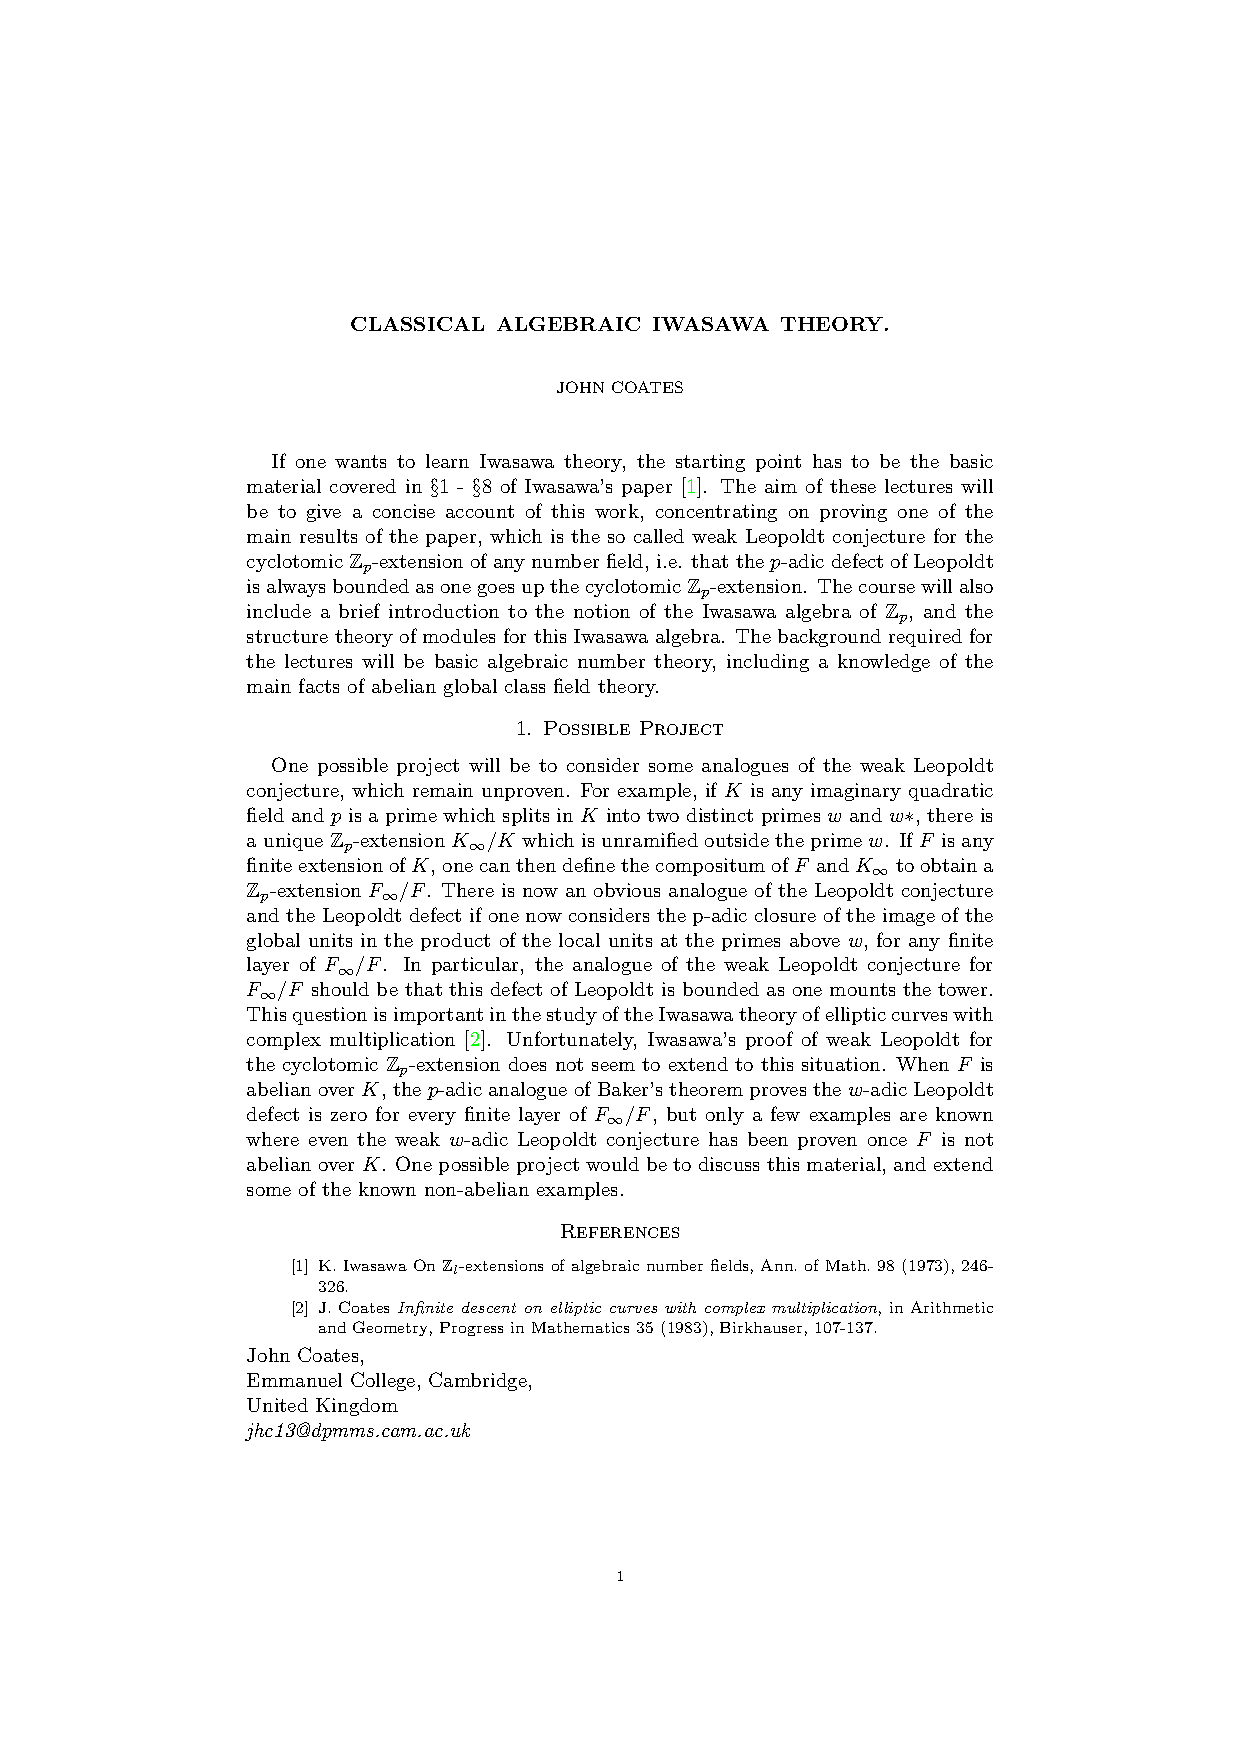
\includepdf[pages=-,scale=1,pagecommand={\thispagestyle{normal}}]{../notes/coates/2018CoatesOutline.pdf}
\addcontentsline{toc}{subsection}{\protect\numberline{\thesubsection} Lecture Notes: Historical Introduction}
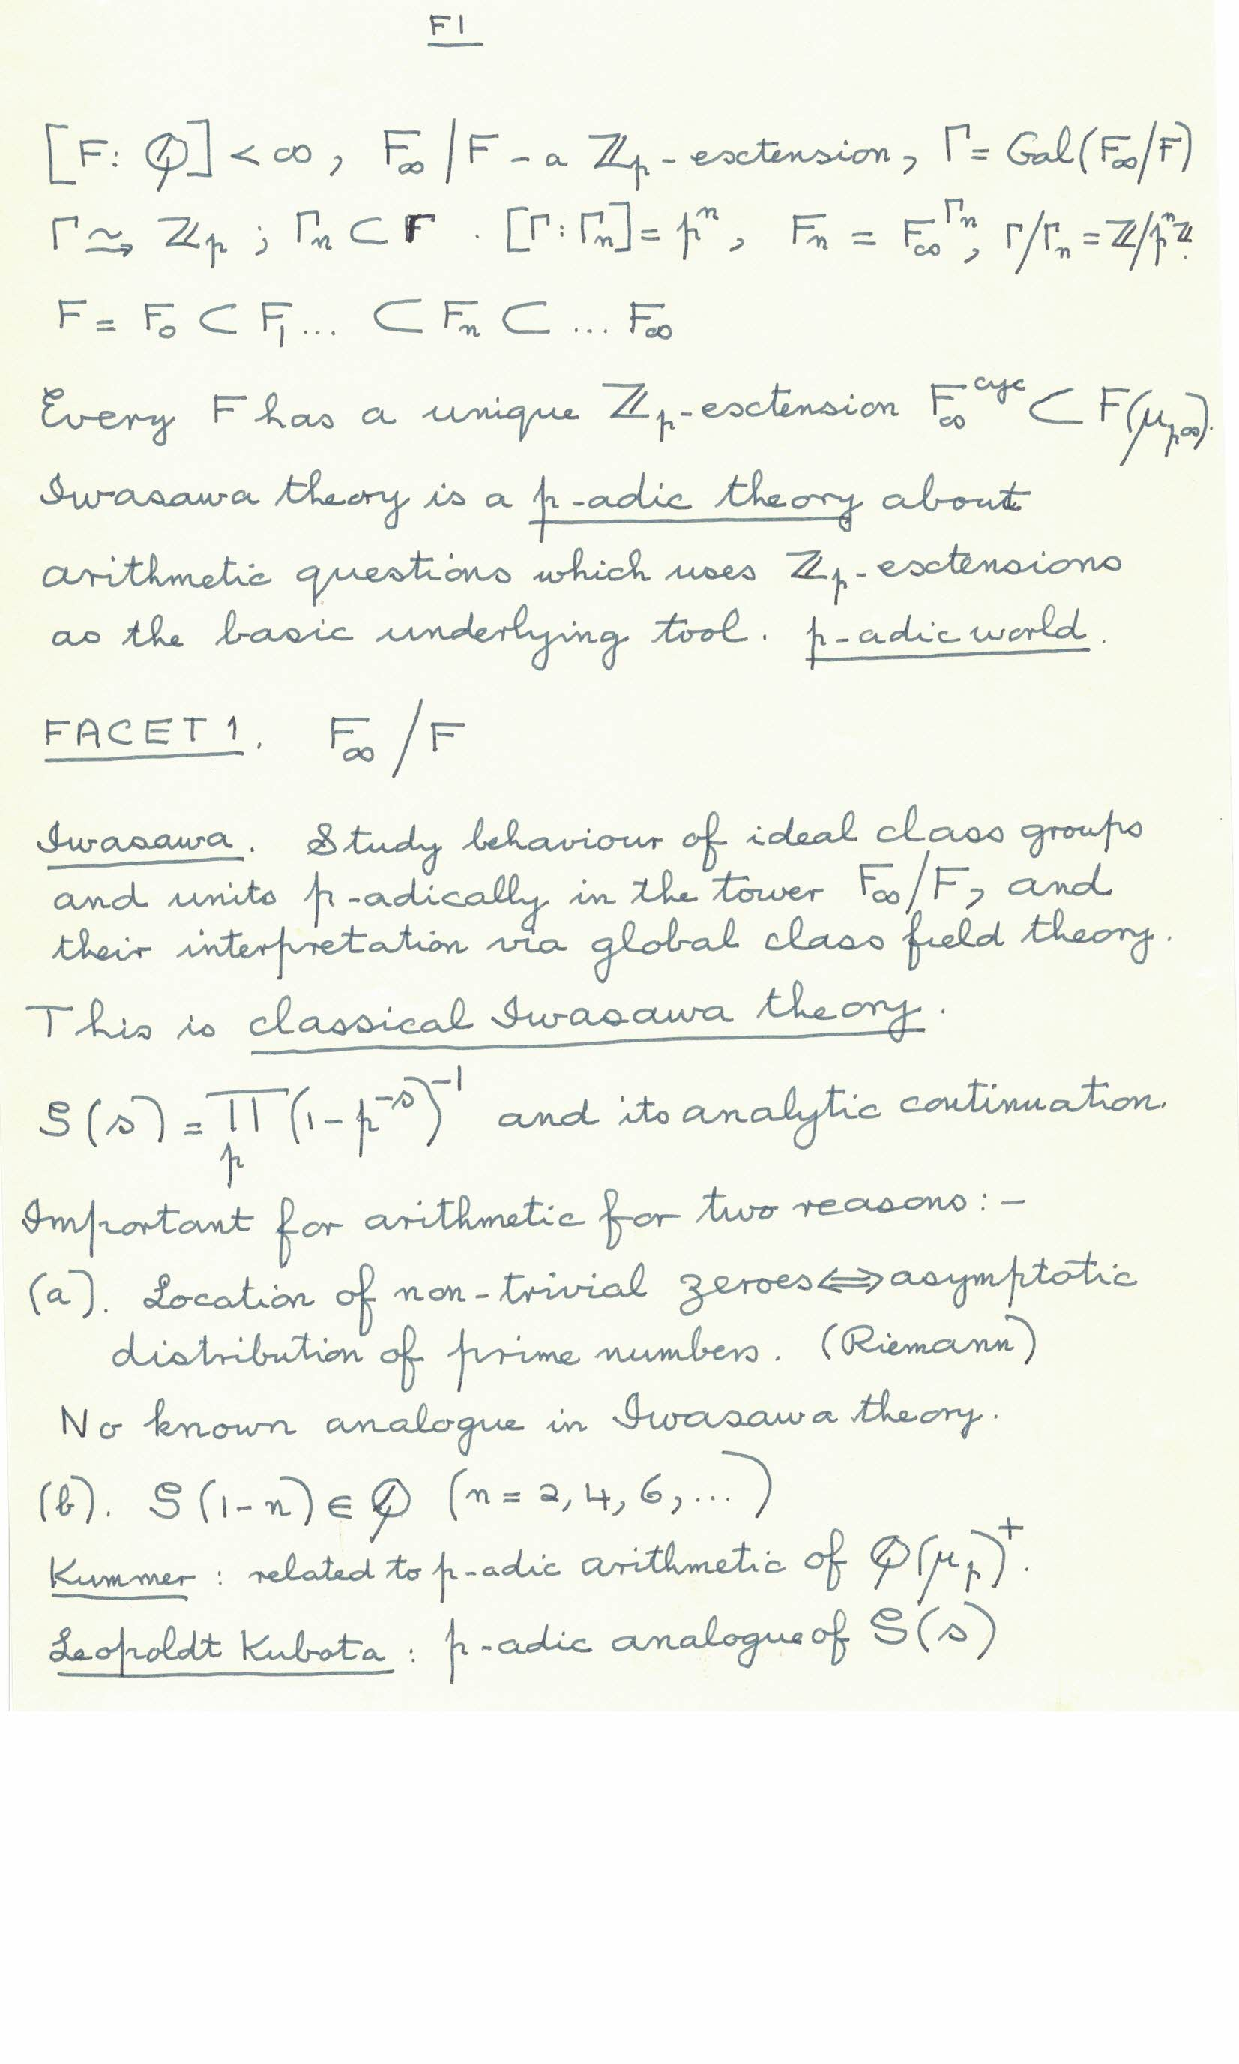
\includepdf[pages=-,scale=1,pagecommand={\thispagestyle{normal}}]{../notes/coates/2018CoatesIntroduction.pdf}
\addcontentsline{toc}{subsection}{\protect\numberline{\thesubsection} Lecture Notes (Original)}
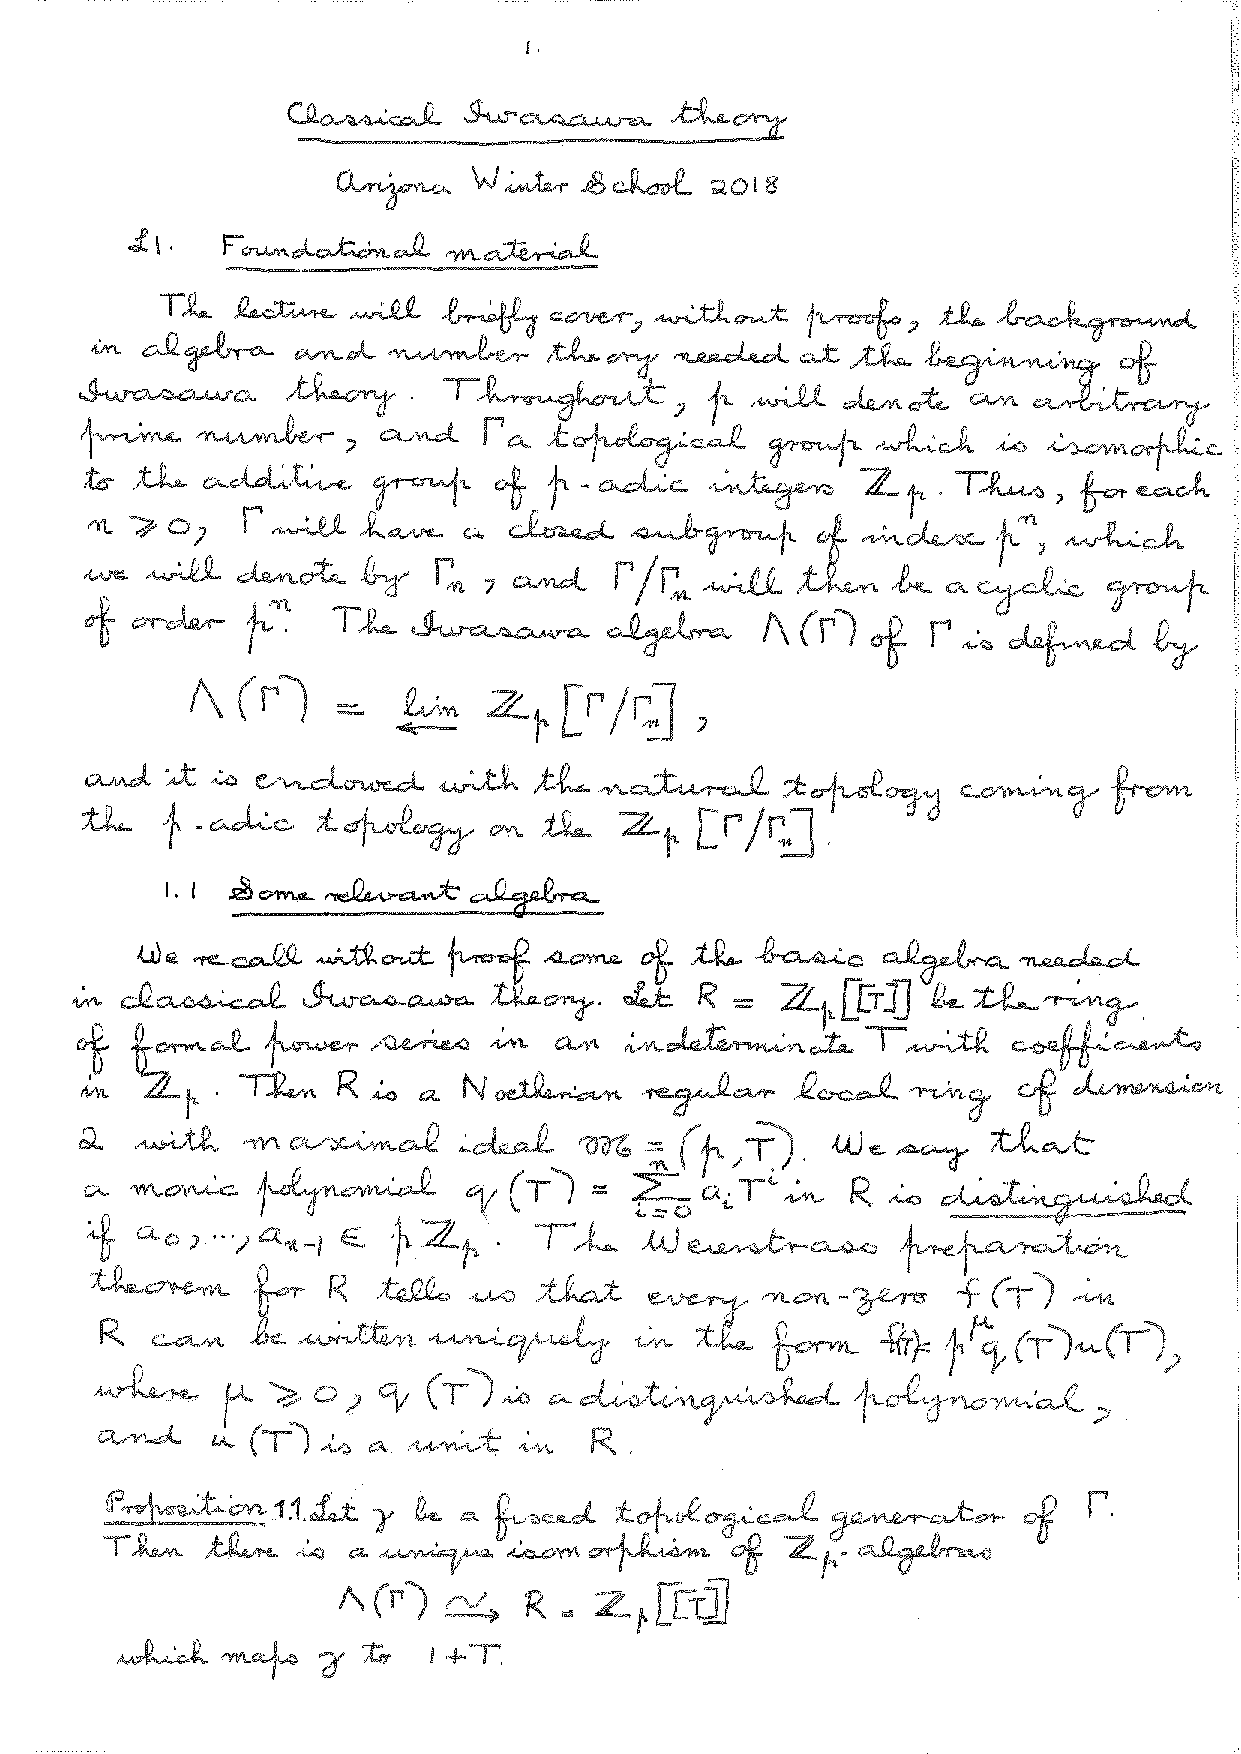
\includepdf[pages=-,scale=1,pagecommand={\thispagestyle{normal}}]{../notes/coates/2018CoatesNotes.pdf}
\addcontentsline{toc}{subsection}{\protect\numberline{\thesubsection} Lecture Notes (Typeset)}
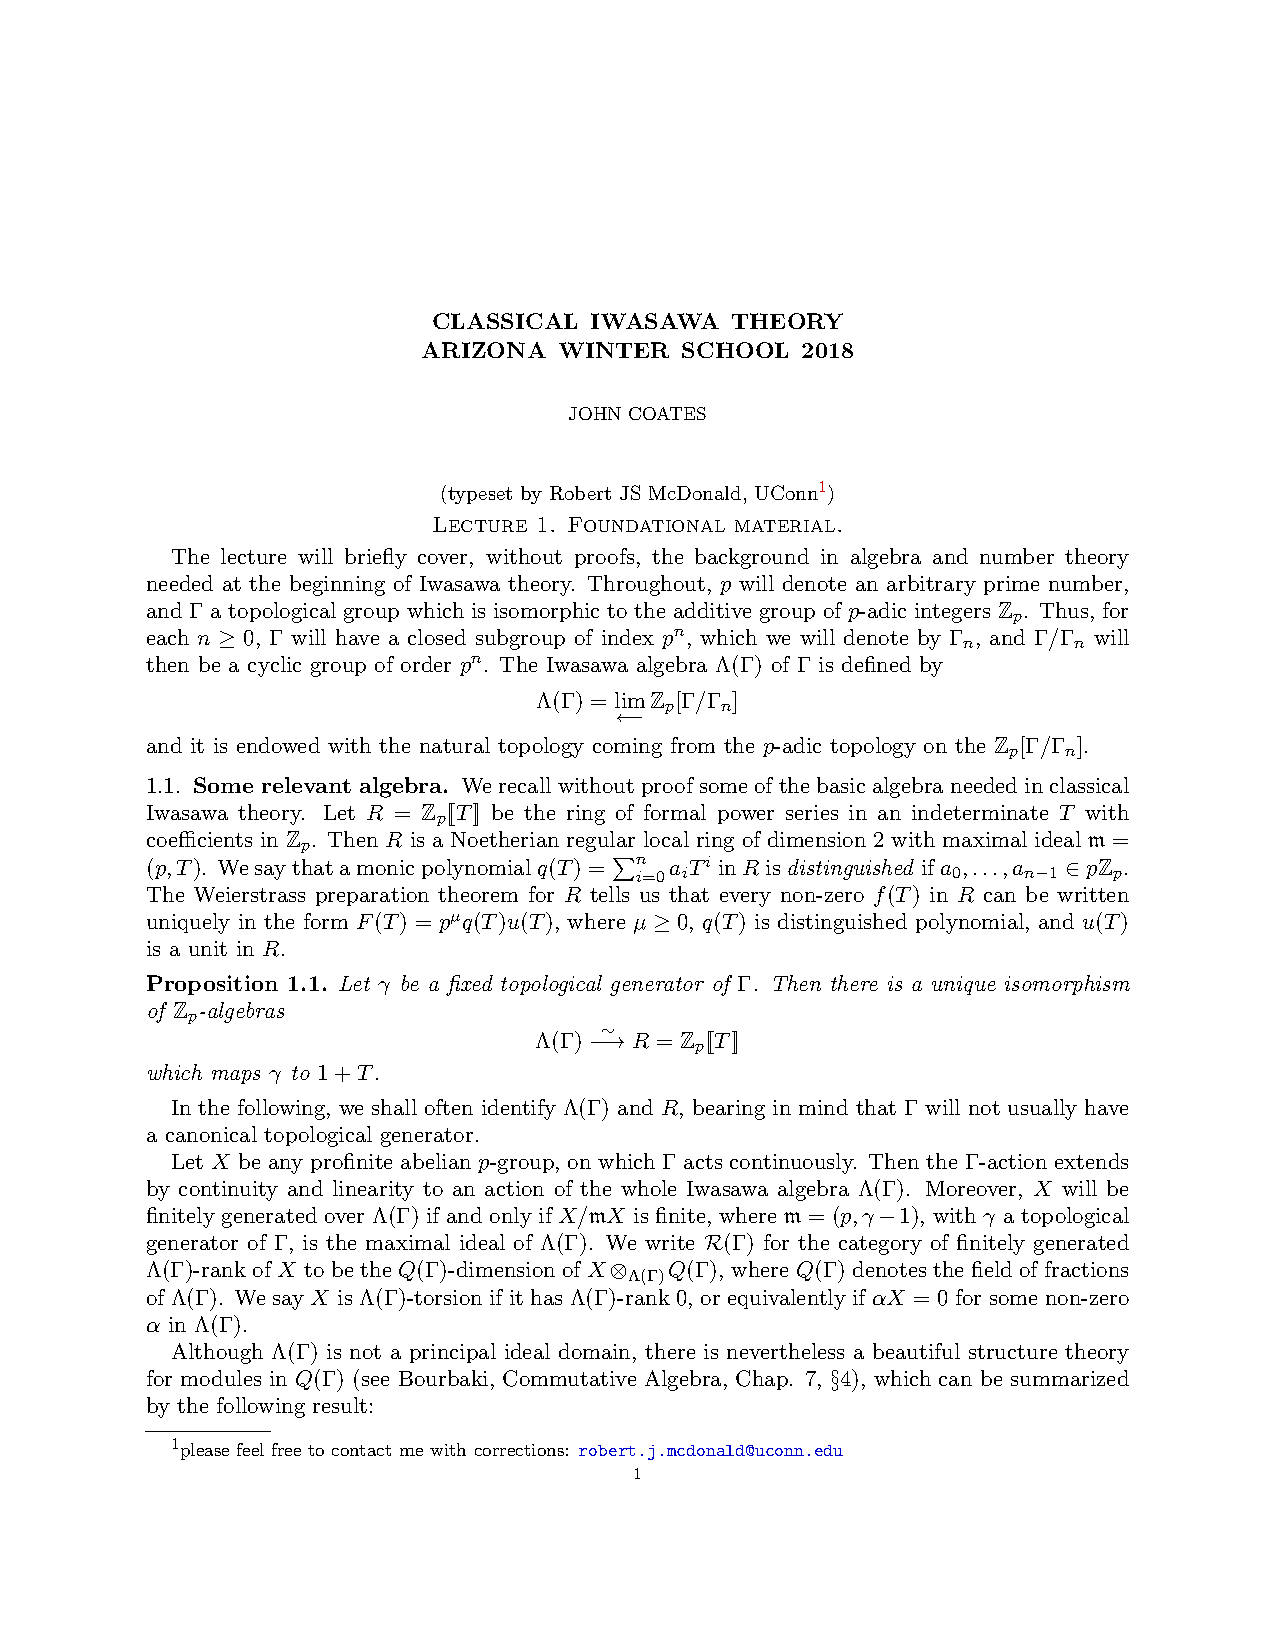
\includepdf[pages=-,scale=1,pagecommand={\thispagestyle{normal}}]{../notes/coates/2018CoatesNotesTypeset.pdf}
\addcontentsline{toc}{subsection}{\protect\numberline{\thesubsection} Project Descriptions}
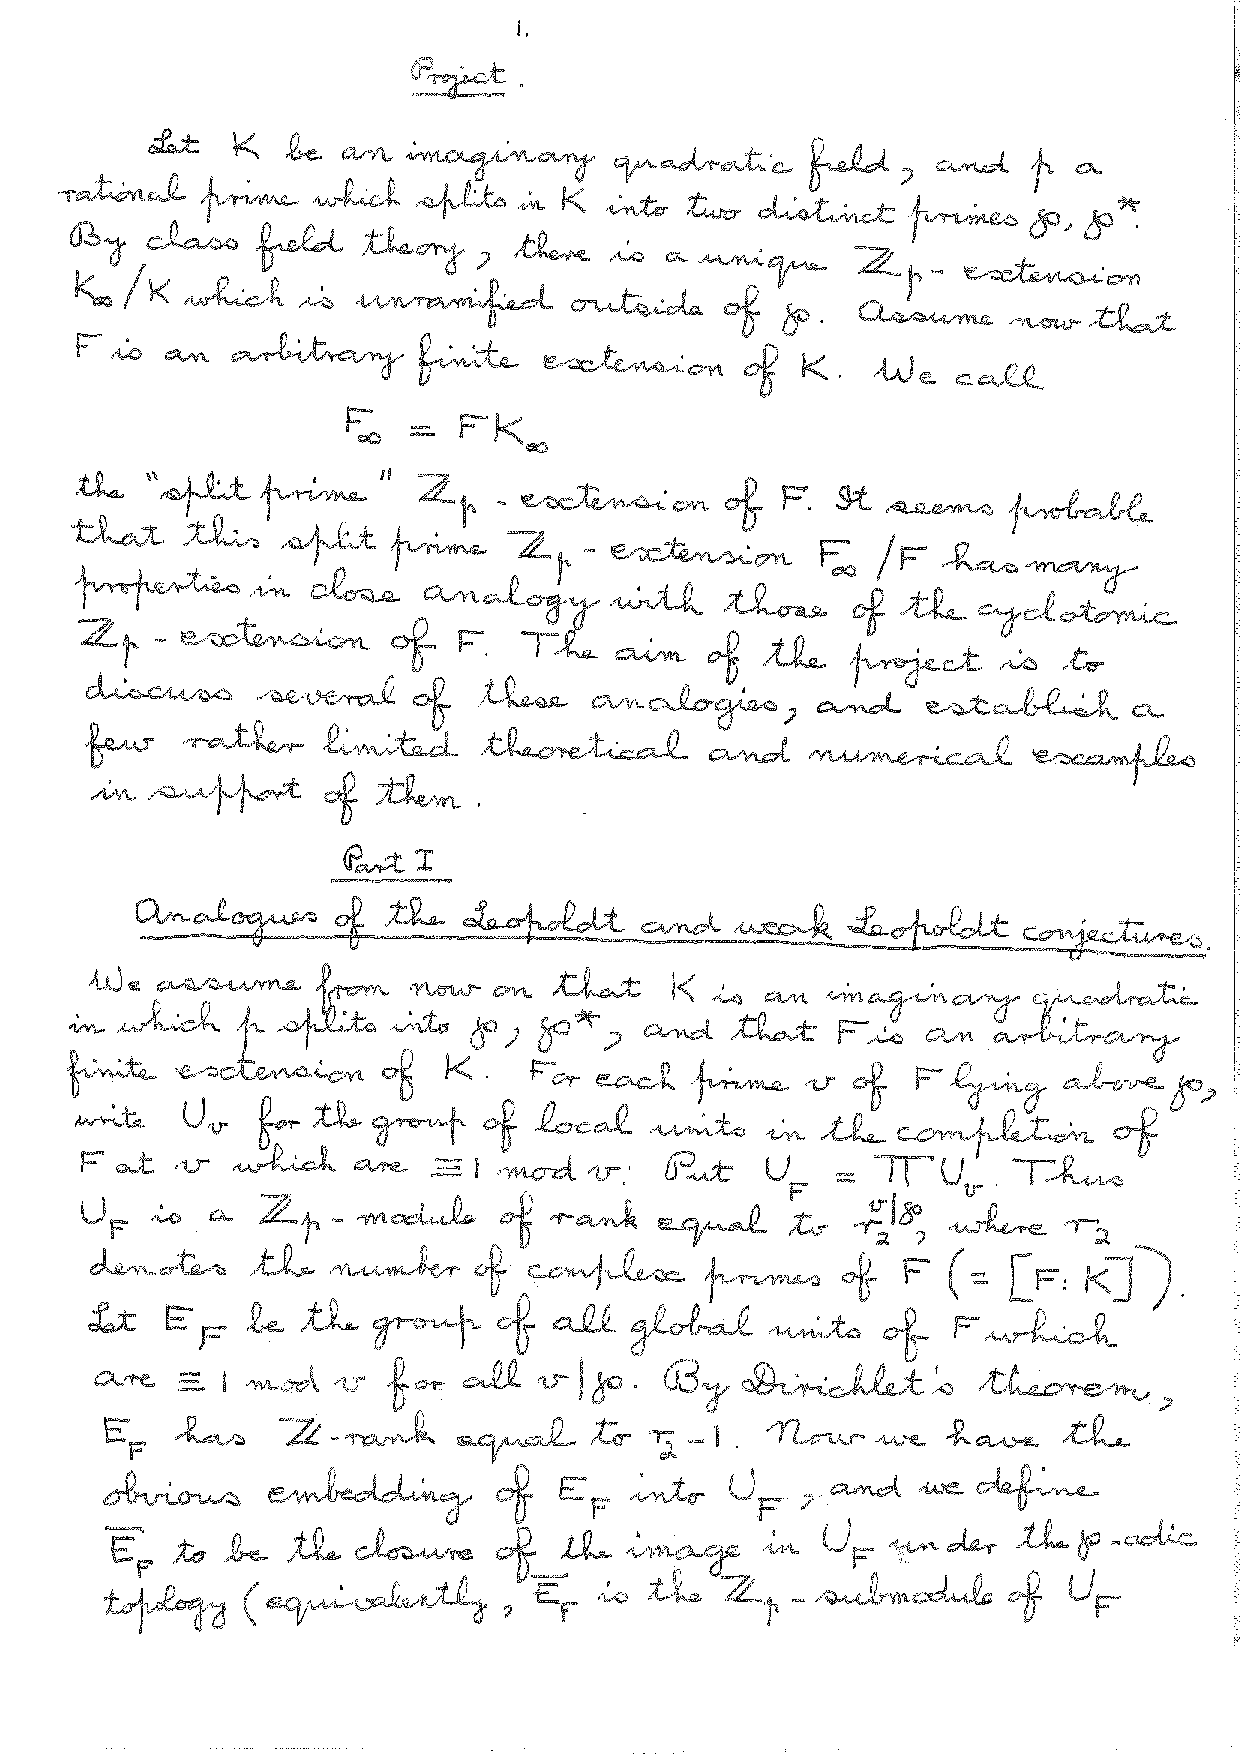
\includepdf[pages=-,scale=1,pagecommand={\thispagestyle{normal}}]{../notes/coates/2018CoatesProject.pdf}

% Loeffler/Zerbes
\phantomsection
\addtocounter{section}{1}
\addcontentsline{toc}{section}{\protect\numberline{\thesection} David Loeffler \& Sarah Zerbes: Euler systems}
\phantomsection
\setcounter{subsection}{1}
\addcontentsline{toc}{subsection}{\protect\numberline{\thesubsection} Course \& Project Outline}
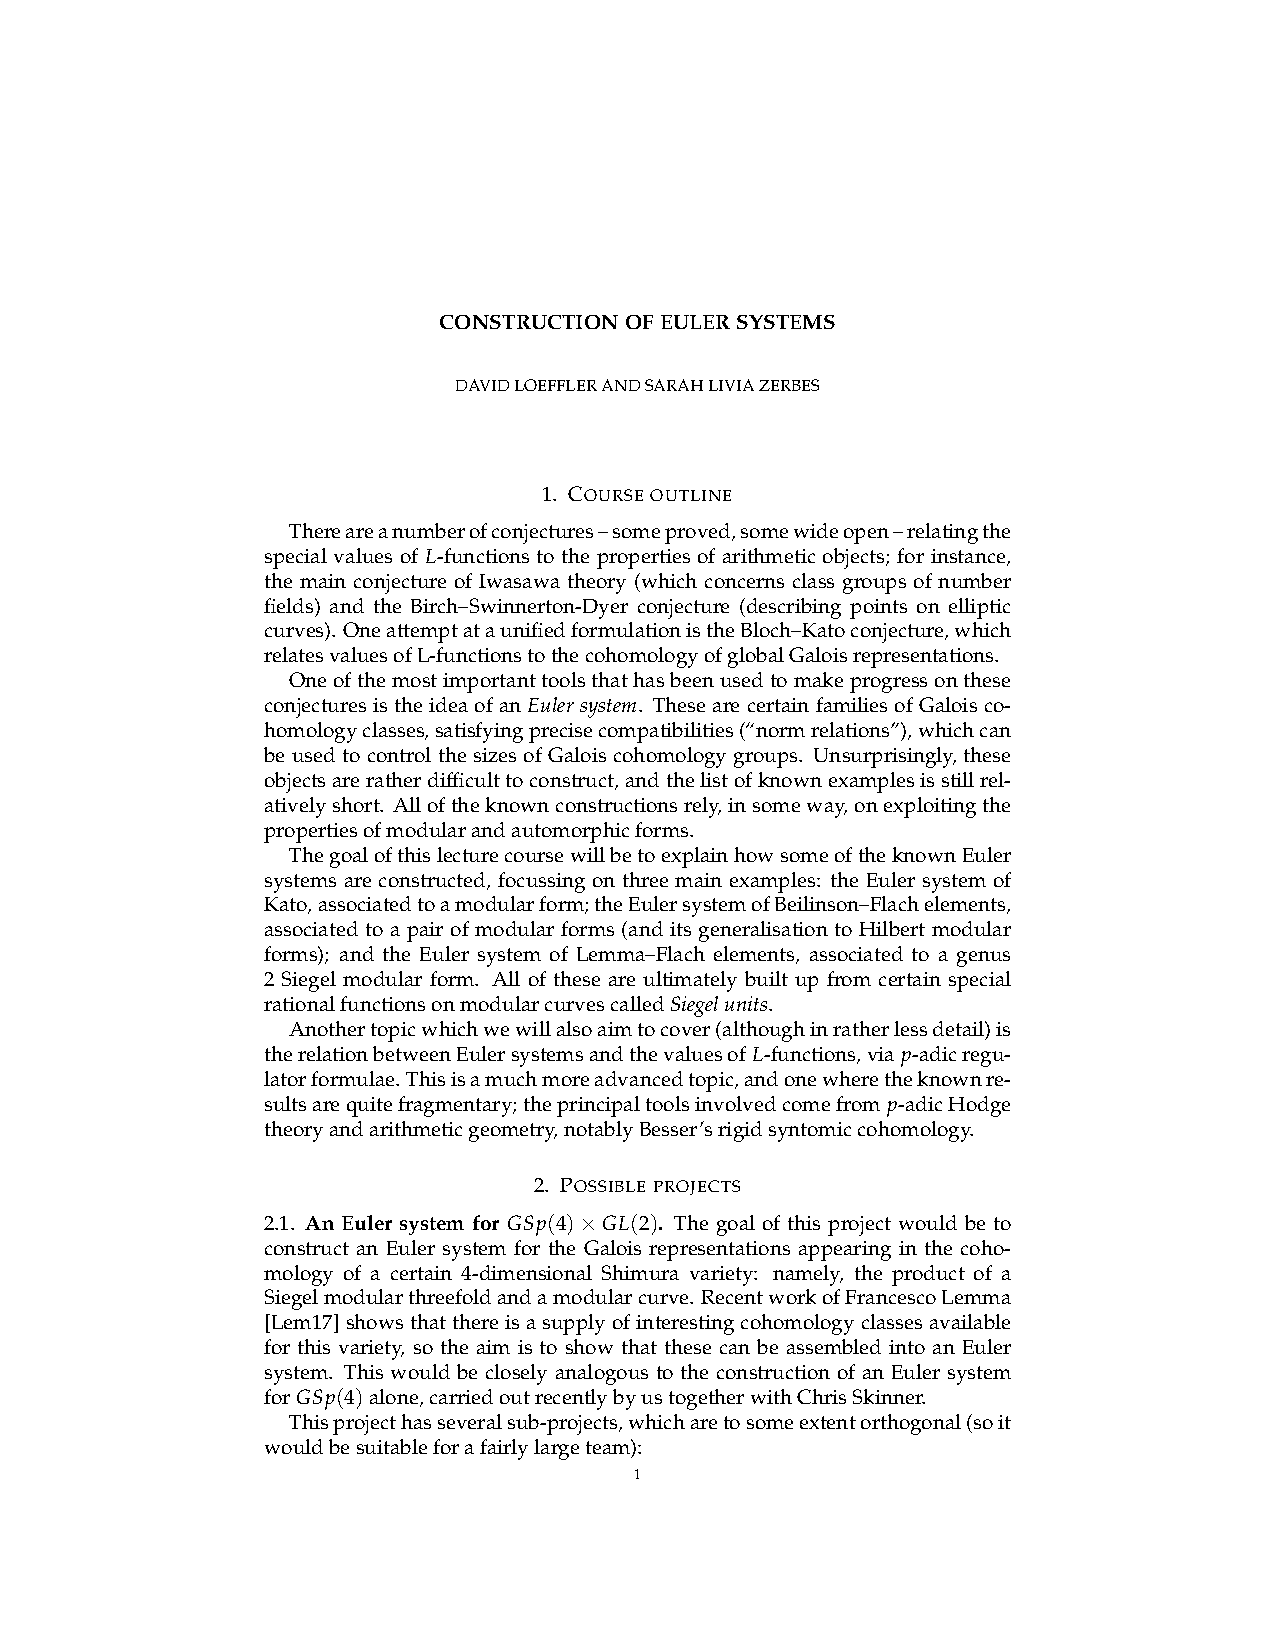
\includepdf[pages=-,scale=1,pagecommand={\thispagestyle{normal}}]{../notes/loeffler_zerbes/2018LoefflerZerbesOutline.pdf}
\addcontentsline{toc}{subsection}{\protect\numberline{\thesubsection} Lecture Notes \& Project Description}

\includepdf[pages=-,scale=1,pagecommand={\thispagestyle{normal}}]{../notes/loeffler_zerbes/2018LoefflerZerbesNotes.pdf}

% Sharifi
\phantomsection
\addtocounter{section}{1}
\addcontentsline{toc}{section}{\protect\numberline{\thesection} Romyar Sharifi: Modular curves and cyclotomic fields}
\phantomsection
\setcounter{subsection}{1}
\addcontentsline{toc}{subsection}{\protect\numberline{\thesubsection} Course \& Project Outline}
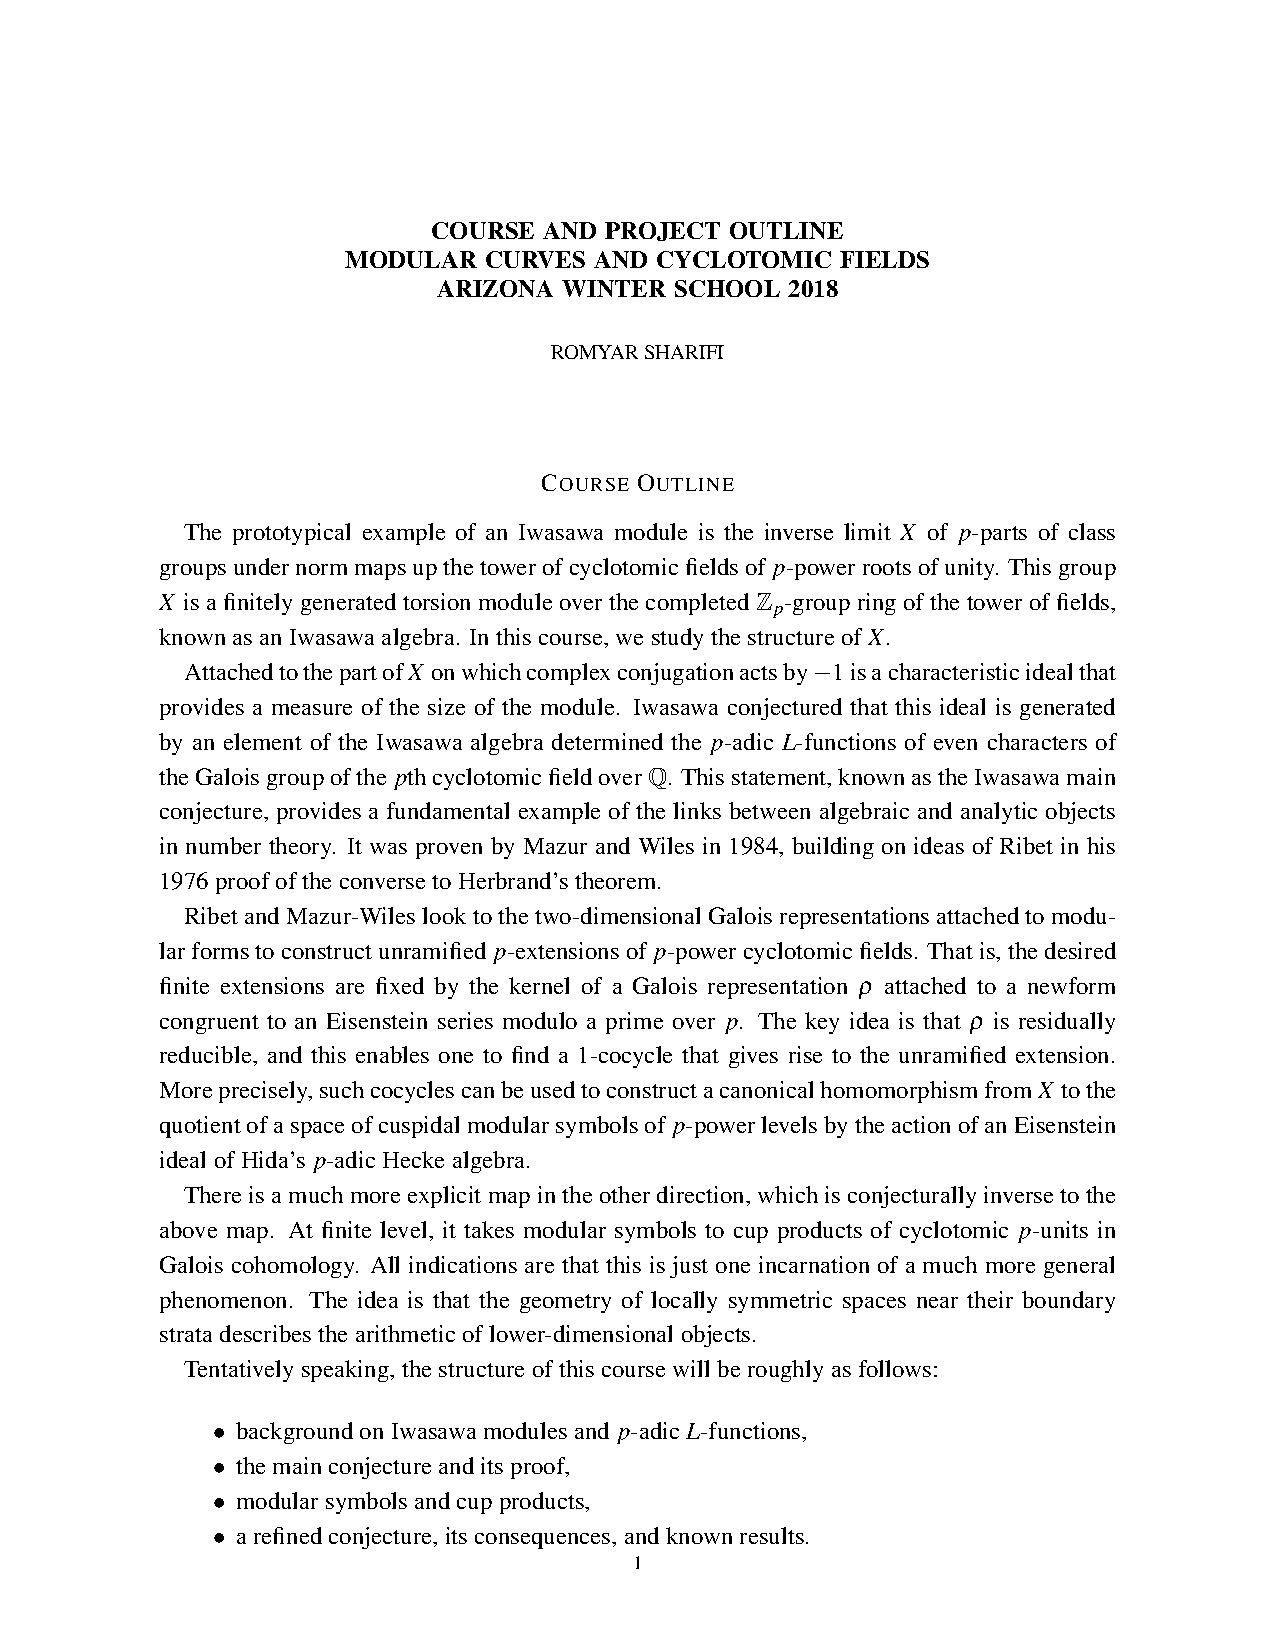
\includepdf[pages=-,scale=1,pagecommand={\thispagestyle{normal}}]{../notes/sharifi/2018SharifiOutline.pdf}
\addcontentsline{toc}{subsection}{\protect\numberline{\thesubsection} Lecture Notes \& Project Description}

\includepdf[pages=-,scale=1,pagecommand={\thispagestyle{normal}}]{../notes/sharifi/2018SharifiNotes.pdf}

% Skinner
\phantomsection
\addtocounter{section}{1}
\addcontentsline{toc}{section}{\protect\numberline{\thesection} Christopher Skinner: Iwasawa theory, modular forms, and elliptic curves}
\phantomsection
\setcounter{subsection}{1}
\addcontentsline{toc}{subsection}{\protect\numberline{\thesubsection} Course \& Project Outline}
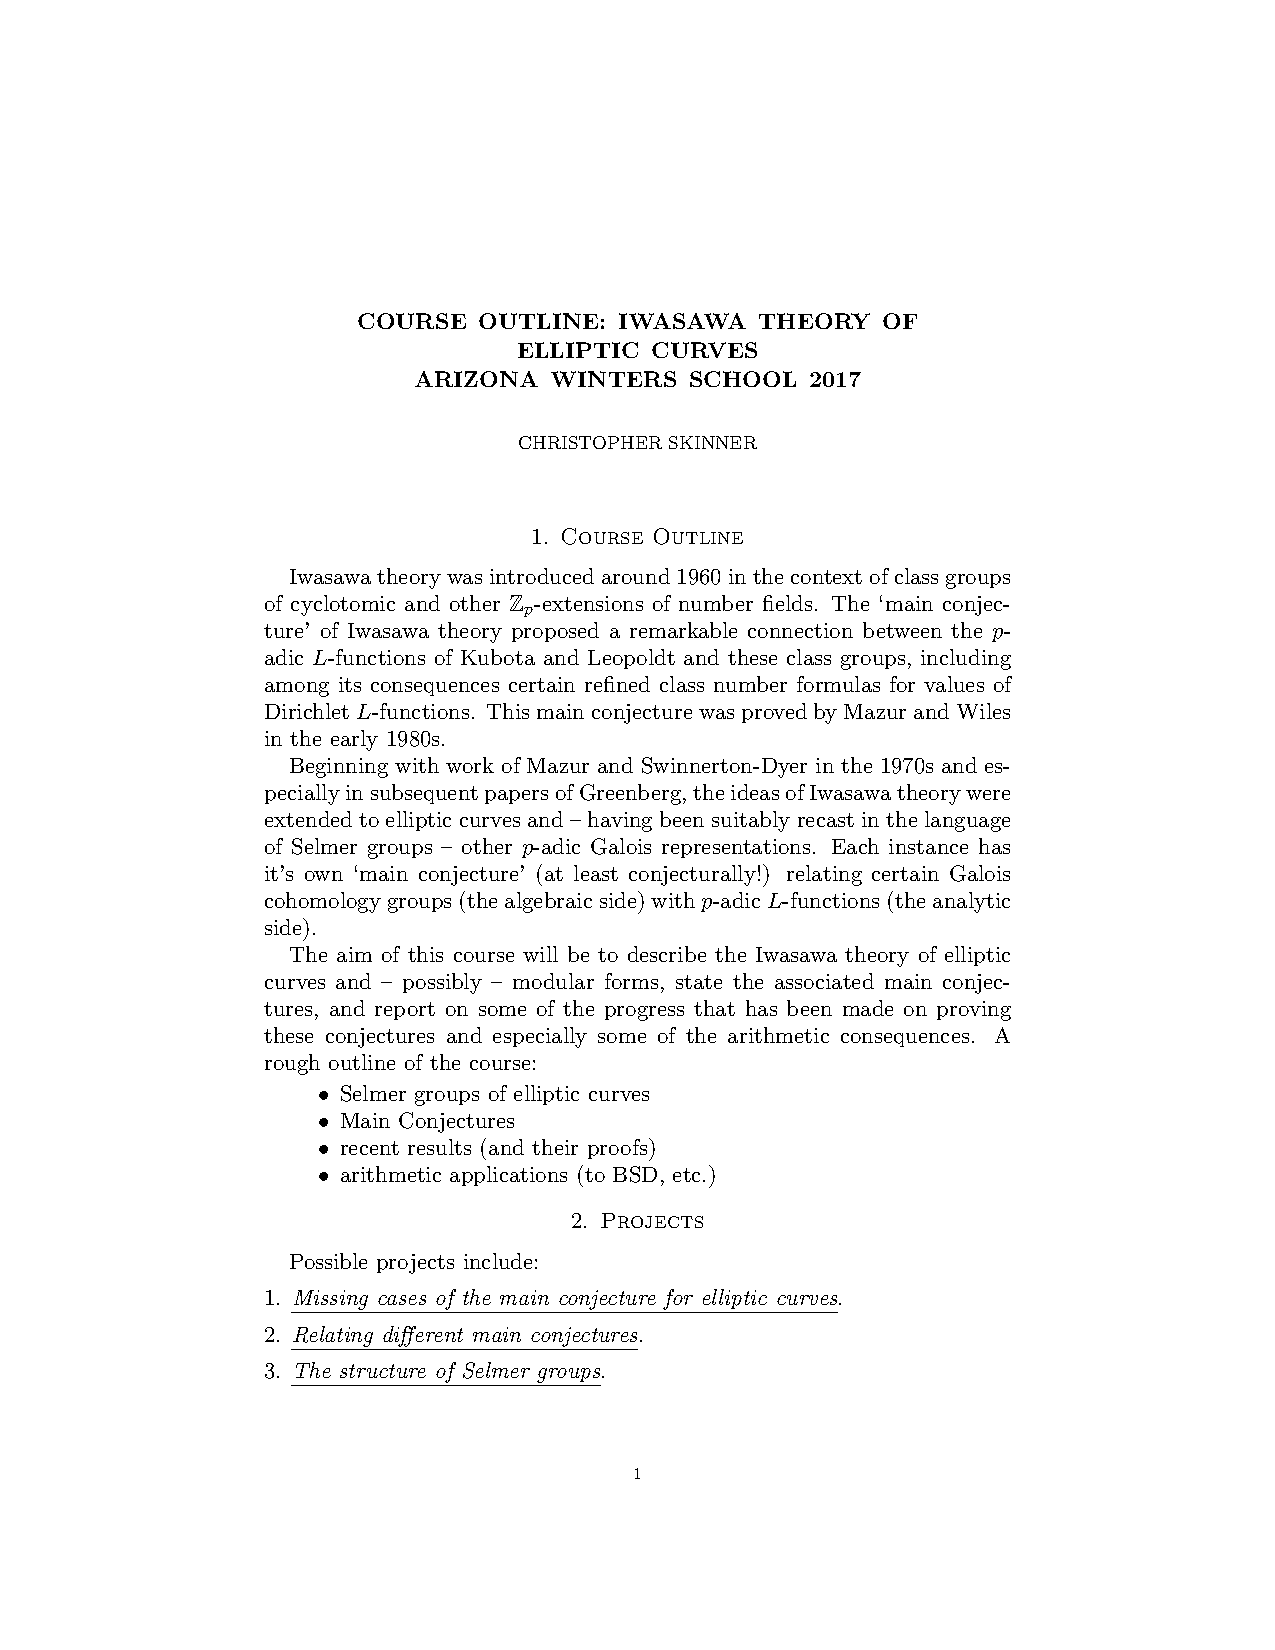
\includepdf[pages=-,scale=1,pagecommand={\thispagestyle{normal}}]{../notes/skinner/2018SkinnerOutline.pdf}
\addcontentsline{toc}{subsection}{\protect\numberline{\thesubsection} Lecture Notes}
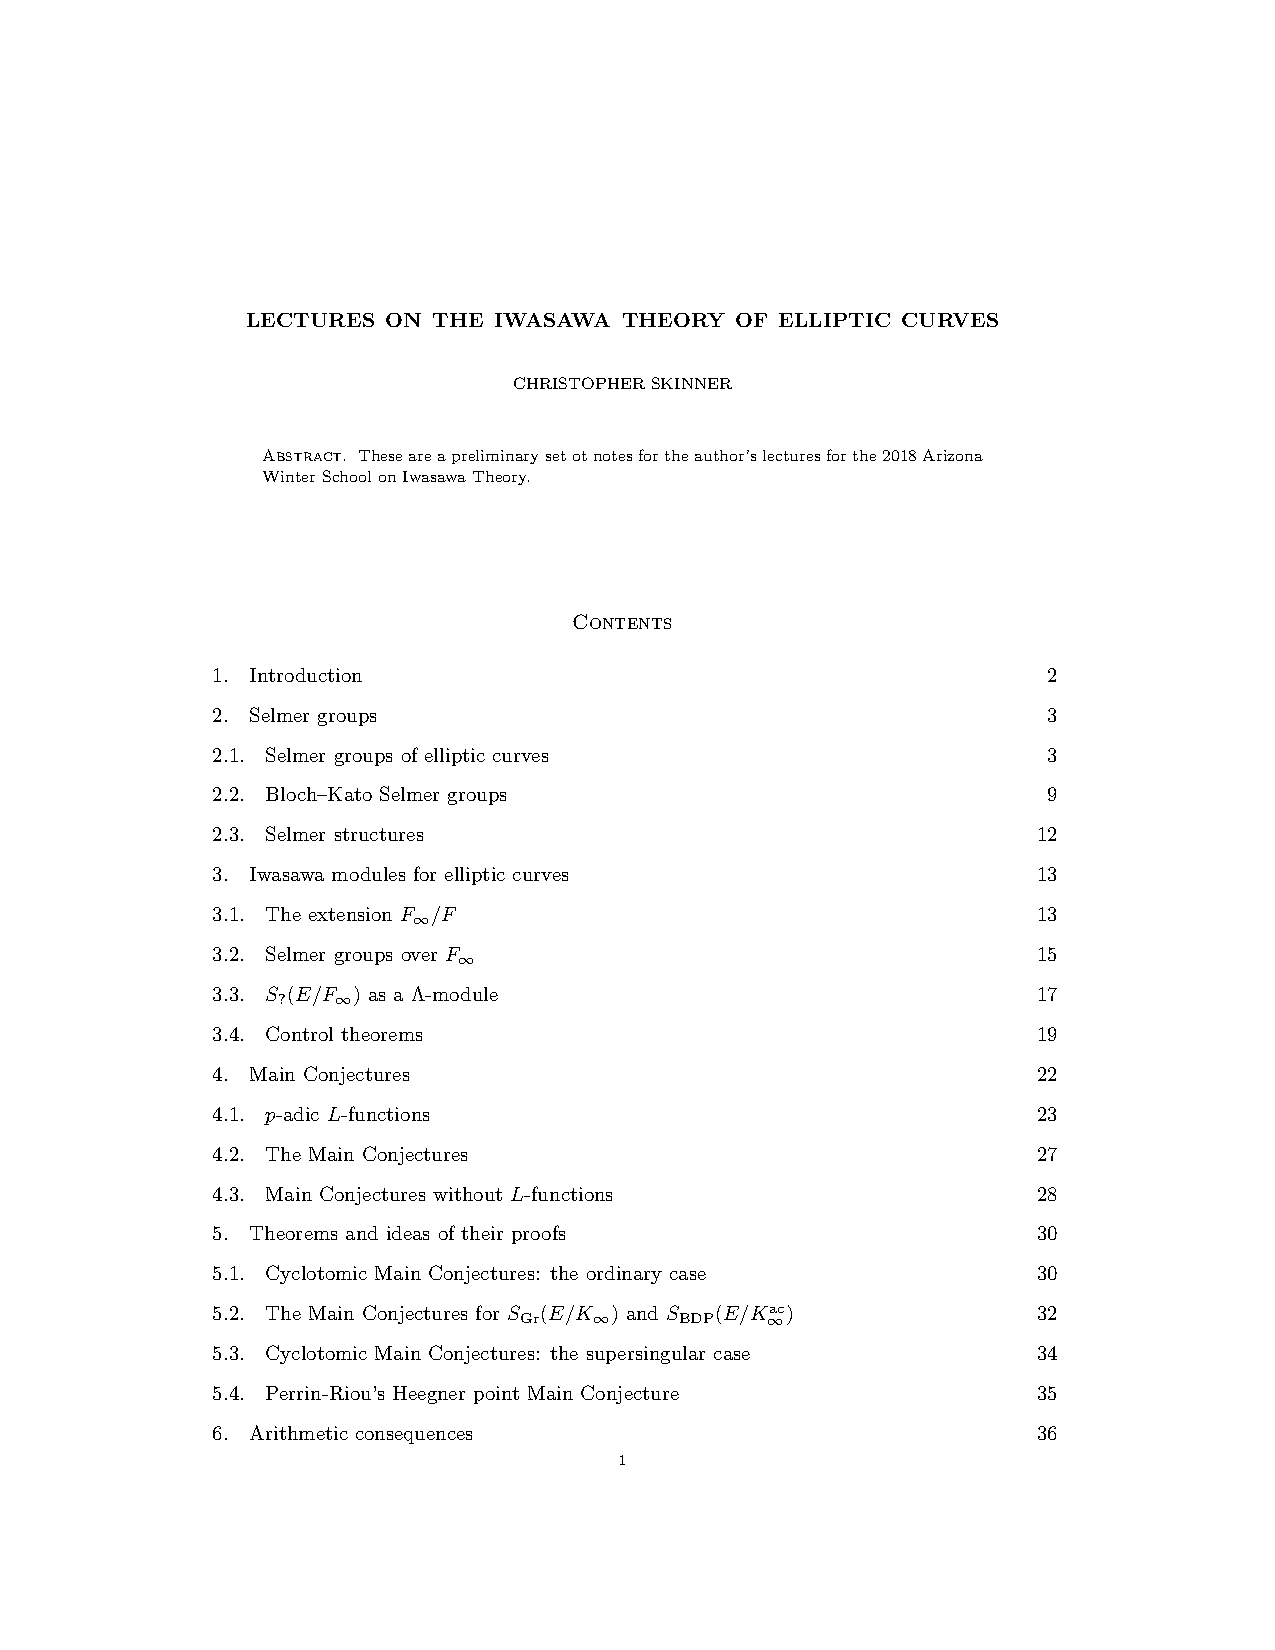
\includepdf[pages=-,scale=1,pagecommand={\thispagestyle{normal}}]{../notes/skinner/2018SkinnerNotes.pdf}
\addcontentsline{toc}{subsection}{\protect\numberline{\thesubsection} Project Description}
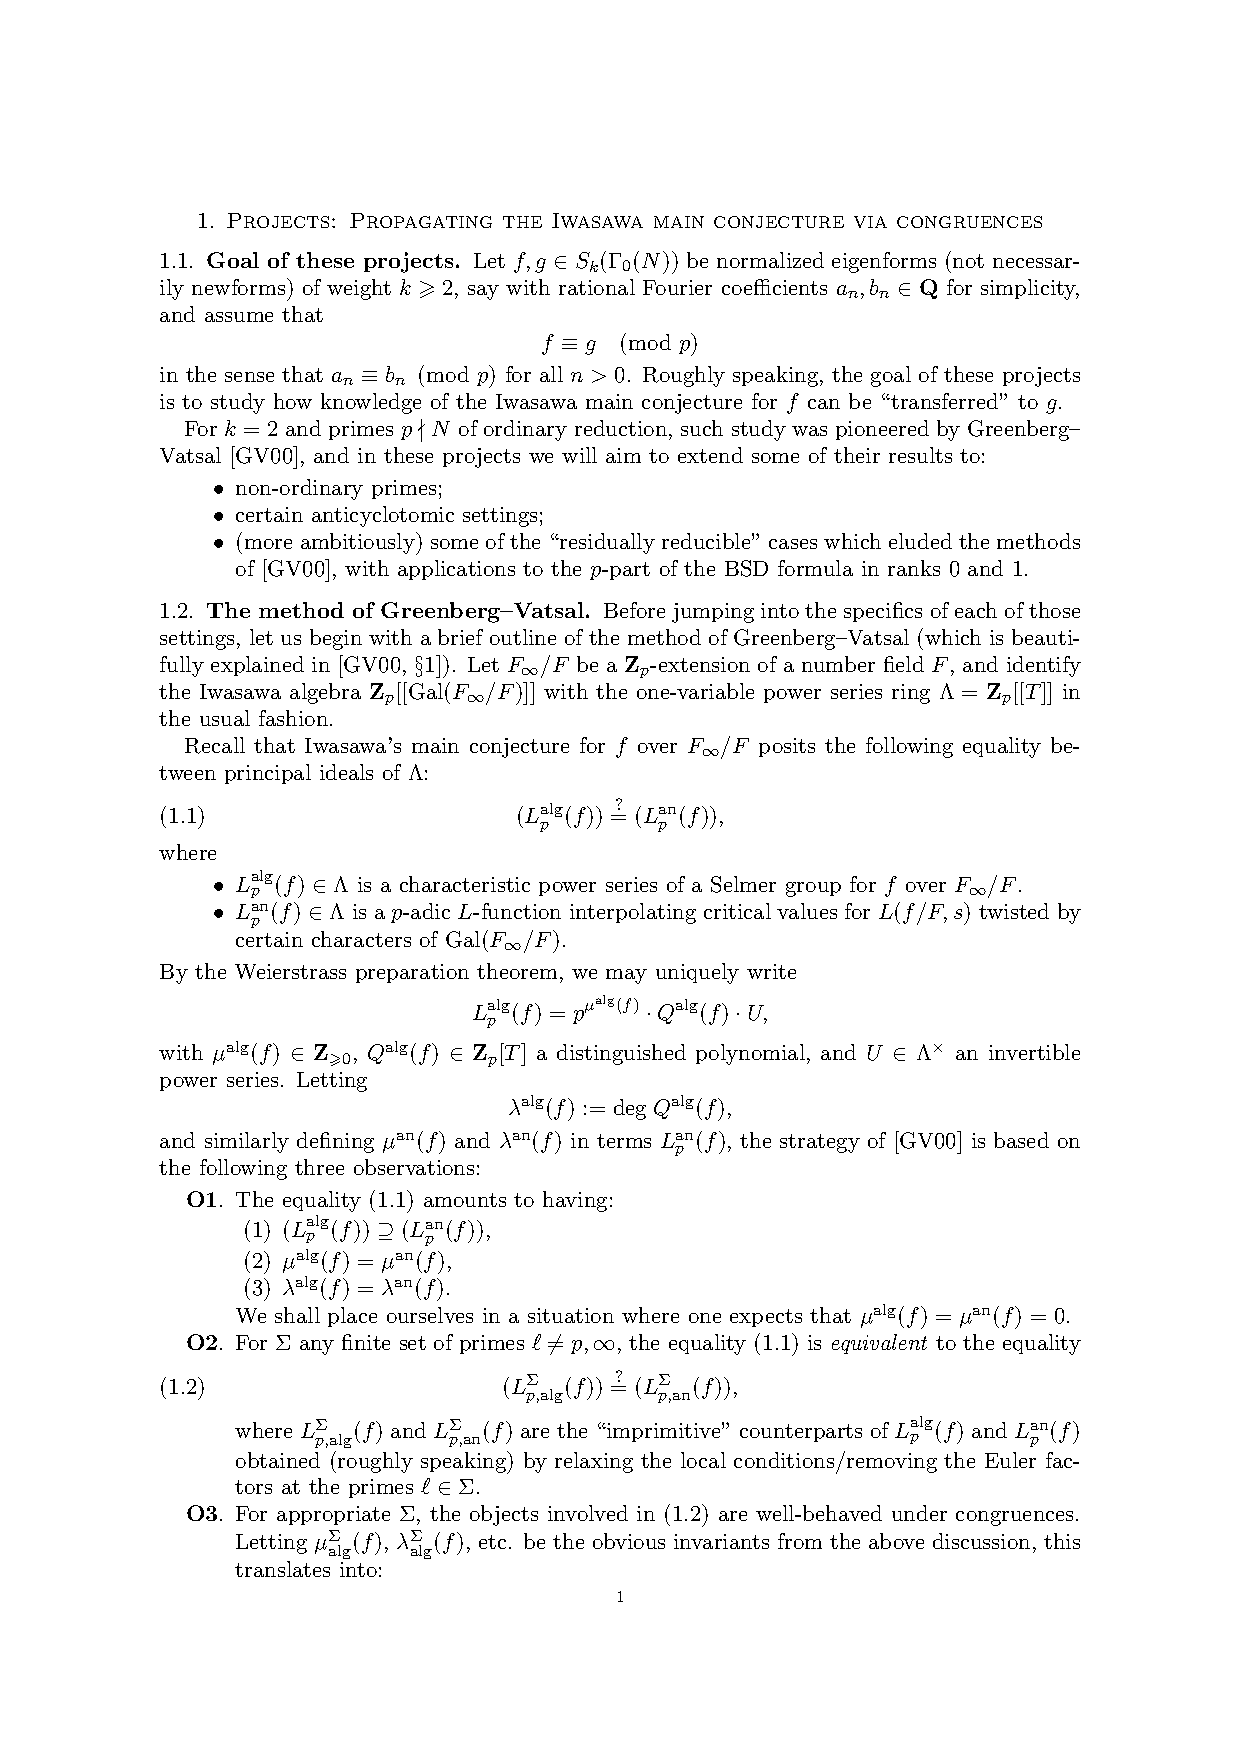
\includepdf[pages=-,scale=1,pagecommand={\thispagestyle{normal}}]{../notes/skinner/2018SkinnerProjects.pdf}
}



% -------------------
% Bibliography
% -------------------
\newpage
\nocite{*}
\printbibliography

\end{document}